%%%%% Beginning of preamble %%%%%
\documentclass[9pt,twocolumn]{extarticle}

%Packages to load which give you useful commands
\usepackage[utf8]{inputenc}
\usepackage{enumerate}
\usepackage{graphicx}
\usepackage[font={footnotesize}]{caption}
\captionsetup[figure]{labelfont=bf}
\captionsetup[table]{labelfont=bf}
\usepackage{subcaption}
\usepackage{mathtools}
\usepackage{amssymb}
\usepackage{verbatim}
\usepackage{placeins}
\usepackage{xspace}
\usepackage{url}
\usepackage{hyperref}
\hypersetup{colorlinks,citecolor=black,filecolor=black,linkcolor=black,urlcolor=black}
\usepackage[titletoc,title]{appendix}
\usepackage{listings}
\usepackage{enumitem}
\usepackage{diagbox}
\usepackage{makecell}
%\usepackage{array,booktabs}
\usepackage{pgfplots}
\DeclarePairedDelimiter{\ceil}{\lceil}{\rceil}
\newcommand\numberthis{\addtocounter{equation}{1}\tag{\theequation}}
\usepackage{wasysym}
\usepackage{lipsum}


%Sets the margins
\textwidth = 7 in
\textheight = 9.5 in
\oddsidemargin = -0.3 in
\evensidemargin = -0.3 in
\topmargin = -0.4 in
\headheight = 0.0 in
\headsep = 0.0 in
%\parskip = 0.2in
\parindent = 0.5in
\textfloatsep = 0.2in

%defines a few theorem-type environments
\newtheorem{theorem}{Theorem}
\newtheorem{corollary}[theorem]{Corollary}
\newtheorem{definition}{Definition}

%lstlistings settings
\lstset{
  language=R,
  basicstyle=\ttfamily\scriptsize,
  numbers=left,
  numberstyle=\tiny\color{black},
  stepnumber=1,
  numbersep=5pt,
  backgroundcolor=\color{white},
  tabsize=2,
  captionpos=b,
  extendedchars=true,
  breaklines=true,
  xleftmargin=.25in,
  xrightmargin=.25in,
    showstringspaces=false
}

% minted framebox
\usepackage[]{minted}
\usepackage{tcolorbox}
\usepackage{etoolbox}
\BeforeBeginEnvironment{minted}{\hspace{-0.5em}\begin{tcolorbox}[]}%
    \AfterEndEnvironment{minted}{\end{tcolorbox}}%

% Lessen paragraph indentation
\setlength\parindent{2ex}

% custom commands
\newcommand{\sympy}{\texttt{SymPy}\xspace}
\newcommand{\floor}[1]{\lfloor #1 \rfloor}
\newcommand{\pvalue}{\textit{p}-value\xspace}
\newcommand{\anova}{\textsc{anova}\xspace}
\newcommand{\ancova}{\textsc{ancova}\xspace}
\newcommand{\norm}[2]{\|#1\|_#2}
\newcommand{\abs}[1]{|#1|}
\newcommand{\minus}{\scalebox{0.75}[1.0]{$-$}}
\newcommand{\cond}{\text{cond}}
\newcommand{\expect}[1]{\mathop{{}\mathbb{E}}[#1]}
\newcommand{\expectt}[2]{\mathop{{}\mathbb{E}_{#1}}[#2]}
\newcommand{\real}{\mathop{{}\mathbb{R}}}
\newcommand{\nat}{\mathop{{}\mathbb{N}}}
\newcommand{\var}[1]{\text{Var($#1$)}}
\newcommand{\varb}[1]{\text{Var\big($#1$\big)}}
\providecommand{\e}[1]{\ensuremath{\times 10^{#1}}}
\newcommand{\len}{\ell}
\newcommand{\sumpx}{\sum_{x \in X}P_X(x)}
\newcommand{\entropy}{\sumpx \cdot \log\frac{1}{P_X(x)}}
\newcommand{\avglen}{\sumpx \cdot \ell(C(x))}
\newcommand{\probset}[3]{{#1}_{#2}^{(#3)}}
\newcommand{\typical}{\probset{A}{\epsilon}{n}}
\newcommand{\smallest}{\probset{B}{\delta}{n}}
\newcommand{\mupos}{\mu_{\text{pos}}}
\newcommand{\muneg}{\mu_{\text{neg}}}
\newcommand{\inner}[2]{\langle #1, #2\rangle}
\newcommand{\tand}{~\text{and}~}
\newcommand{\tor}{~\text{or}~}
\newcommand{\limninf}{\lim\limits_{n \to \infty}}
\newcommand{\vect}[1]{\boldsymbol{#1}}
\newcommand{\book}{book by Eiben and Smith \cite{eiben2003introduction}\xspace}

\def\app#1#2{%
    \mathrel{%
        \setbox0=\hbox{$#1\sim$}%
        \setbox2=\hbox{%
            \rlap{\hbox{$#1\propto$}}%
            \lower1.1\ht0\box0%
        }%
        \raise0.25\ht2\box2%
    }%
}
\def\approxprop{\mathpalette\app\relax}
\pgfplotsset{compat=1.12}
%%%%% End of preamble %%%%%


\begin{document}

\title{Evolutamine: Evolutionary Computing\\
  \small Computational Science - Vrije Universiteit Amsterdam}

\author
{
    Martijn van Beest\\
    \small{fbt600@student.vu.nl}\\
    \small{1620746}
    \and
    Rahiel Kasim\\
    \small{rkm700@student.vu.nl}\\
    \small{2184532}
}
\date{20 October 2017}
\maketitle


\section{Introduction}
We were given three 10-dimensional functions and were tasked with designing and implementing an
algorithm to find their global maxima. Each function has a domain consisting of 10 real numbers:
$x_1, x_2, \ldots x_{10}$ where $x_i \in [-5, 5] \subset \mathbb{R}$. The functions return a value
in $[0, 10] \subset \mathbb{R}$ that signifies the closeness to the maximum where a larger value is
closer and a value of 10 corresponds with the maximum. This problem as described is a constrained
optimisation problem (COP). For every function there is an evaluation limit: the maximum number of
times the function is allowed to be evaluated by the algorithm.

Finding the maxima by brute-force is infeasible: because the inputs are real numbers, the number of
possible inputs are uncountably infinite. Given such an enormous search space we desire an algorithm
that terminates within polynomial time and finds a ``good enough'' solution i.e. close enough to the
maximum. These requirements can be fulfilled by an evolutionary algorithm (EA).

In this report we describe the design and implementation of our EA. Our main reference was the
text\book.

The provided functions are Bent Cigar, Katsuura and Schaffers F7. An interesting property that both
the Katsuura and the Schaffers F7 function posses is multimodality. After a description of our
methodology in section \ref{sec:methodology} we will expand on the multimodality property in section
\ref{sec:multimodality}.

\section{Methodology}\label{sec:methodology}
Because there is no single EA that works perfectly for all problems, our approach was to start with
a simple EA and to experiment with the individual components. In general an EA has a set number of
components that differ between algorithms: parent selection, recombination, mutation and survivor
selection. We have tried different methods for each of these components and eventually settled on
the combination of methods that produced the best results.

The first step in designing an EA is deciding on a representation of individuals. For our problem
there is a very natural mapping between phenotypes and genotypes. Our phenotypes are tuples of 10
real numbers ($x_1, x_2, \ldots x_{10}$) that comprise the input to a function. Real numbers have
infinite precision while numbers represented on computers usually have finite precision. There are
methods so computers can compute with numbers of arbitrary precision, but this will be large trade
of performance for precision. We've instead chosen to represent the real numbers as double-precision
floating-point numbers. This format is standardized by the IEEE and double-precision floating-point
arithmetic is supported by most common processors, so it is fast \cite{floats}.

Note that this encoding of phenotypes to genotypes is surjective but not injective: (infinitely)
many phenotypes are mapped to the same genotype. We don't consider this an issue as the precision of
doubles is at around 15 decimal digits for numbers in the range $[-5, 5]$ \cite{wiki:floats}.

For the initialization of the EA we start with a population of some size and provide each individual
with 10 uniformly sampled doubles (genes) in the range $[-5, 5]$. The evolution of the population is
described in the following sections.

\subsection{Parent Selection}
Our first step in the evolutionary cycle is the selection of individuals that will reproduce to
create offspring. Most of the methods we have implemented base the selection on the fitness of the
individuals. We calculate the fitness of individuals with the provided fitness function.

\subsubsection{Fitness Proportional Selection}
In a first attempt to write an EA, \emph{fitness proportional selection} (FPS) was used. This
method calculates a probability for each individual to be selected for the mating pool by dividing
the individuals fitness by the total fitness of the entire population. Hence, the fittest
individual is most likely to be chosen for reproduction. The parents are then sampled
independently. A known drawback of FPS is \emph{premature convergence}, where a few fit individuals
take over the entire population. This phenomenon immediately occurred in our population. Since our
initial population is random, their fitness is very bad. There is however always an individual that
is bad, but still significantly better than the other individuals. This
individual gets sampled for the mating pool every time, due to its probability close to 1. Without
advanced recombination or mutation, the population does not even change anymore.

\subsubsection{Ranking Selection}
To overcome the problem of premature convergence, we implemented \emph{ranking selection} (RS).
This method still samples individuals with some probability, but the probability does not depend on
the absolute fitness of the individual anymore. The probability is rather based on the rank of the
individual in the population. Ranks are distributed by sorting the population based on their
fitness. The fittest individual acquires rank 1, the least fit individual acquires rank $n$, where
$n$ is the population size. The rank is then mapped to a probability by either a linear
\eqref{eq:linrs} or an exponential ranking function \ref{eq:exprs}.

\begin{align}
\label{eq:linrs}P_{\text{lin-rank}} &= \frac{(2-s)}{\mu} + \frac{2i(s-1)}{\mu(\mu-1)}\\
\label{eq:exprs}P_{\text{exp-rank}} &= \frac{1-e^{-i}}{c}
\end{align}


\subsection{Recombination} \label{sec:recombination}
We've experimented with all of the recombination methods described in section ``4.4.3 Recombination
Operators for Real-Valued Representation'' of the book by Eiben and Smith
\cite{eiben2003introduction}. In the following the arithmetic average of $x$ and $y$ means $\alpha x
+ (1 - \alpha) y$ with some chosen $\alpha$. In our experiments the value of $\alpha$ was uniformly
chosen from $[0, 1]$ for each recombination.

The first method is called ``Simple Arithmetic Recombination''. Given two equal length vectors of
size $n$, we choose a recombination point $k \in [1, n - 1]$. Child 1 inherits the first $k$ values
of parent 1 and the following $(n - k)$ values are the arithmetic averages of the parents. Child 2
receives its first $k$ values from parent 2 and the rest is the same as for child 1.

The second method ``Single Arithmetic Recombination'' is simpler. We pick a random position $k \in
[1, n - 1]$ and the children receive the arithmetic average of their parents' value at position $k$.
The values at all other positions are directly inherited from their parents (child 1 gets the values
of parent 1 and child 2 of parent 2).

The method we ended up using is called ``Whole Arithmetic Recombination''. Here all the values of
the children are the arithmetic averages of the values of the parents. Note that the children are
not identical unless $\alpha = 0.5$ (or if the parents are identical).

The final method discussed in this section is the ``Blend Crossover''. Here the idea is that with
usual recombination, the value of the children is somewhere between the values of the parents. While
with this crossover the children can obtain values outside of the range of their parents. This
provides more exploration for an EA. After implementing this method we saw no (significant) increase
in the score, so we opted to use the simpler ``Whole Arithmetic Recombination'' method instead.

\subsection{Mutation} \label{sec:mutation}
For mutation we've evaluated the methods described in the section ``4.4 Real-Valued or
Floating-Point representation'' of the \book. As the
methods described in this section increased in complexity as the text continued, so did the EA
achieve better results for our problem. We've implemented all the mutations except ``Correlated
Mutations'' and selected ``Uncorrelated Mutation with $n$ Step Sizes'' due to its superior results.

The section starts out with a simple method called ``Uniform Mutation'' where the idea is to reset a
value with a new uniformly drawn number. This method is quite destructive as any correlation with
the previous value is lost. A more gentle method with better results is ``Nonuniform Mutation'',
here the value is drawn from a Gaussian distribution with a standard deviation or mutation step size
$\sigma$ with zero mean. The new values are normally close to the previous values, but larger
deviations are still possible.

A better method still is ``Uncorrelated Mutation with One Step Size'', where the mutation rate
itself becomes a parameter subject to evolution. In this mutation mechanism first the mutation rate
is mutated and then this new rate is used for the mutation of the actual values of interest. This
order is important: by using the new mutation rate in the mutation the following fitness test of the
new individual is also a fitness test of the new mutation rate. In this method the same mutation
rate $\sigma$ is used for all dimensions.

The last improvement towards our final method employs a different $\sigma_i$ for each dimension
$x_i$ in the method called ``Uncorrelated Mutation with $n$ Step Sizes''. Here each individual has
$2n$ parameters in evolution: its $n$ values $x_i$ and the related $n$ mutation rates $\sigma_i$.
The insight here is that different dimensions don't necessarily correlate, so they are provisioned
with independent mutation rates.

The ``Correlated Mutations'' method takes the self-adaptation of the mutation even further by having
the direction of mutation in the phase space as evolvable parameters. This is accomplished by
introducing $n_\alpha= \frac{n \cdot (n - 1)}{2}$ parameters $\alpha_i$ that specify the mutual
angles between all $n$ dimensions. The total number of parameters under evolution would then be:
$2n+ \frac{n \cdot (n - 1)}{2} = \frac{n^2 + 3n}{2}$. This is a substantial increase in variables to
evolve, and here one has to really consider if it is worth. Because if we have more evolution
parameters, the algorithm has more options to consider and so more evaluations are needed to adapt
to the fitness function. This is a disadvantage given our evaluation limit. More importantly, this
method samples random vectors from a n-dimensional Gaussian, an algorithm absent from Java's
standard library. We were unable to import the \mintinline{java}{MultivariateNormalDistribution}
class from the Apache Commons library \cite{wiki:commons} due to unfamiliarity with the Java
ecosystem and thus we could not implement this mutation mechanism.

\subsection{Survivor Selection}
In our first approach we used a generational model as a replacement strategy. This was the simplest
way to complete a full evolutionary cycle. In later versions, we switched to a more sophisticated
fitness-based method to select surviving individuals. Both ($\mu+\lambda$) and ($\mu,\lambda$)
selection were considered, but since we had to work with a limited number of evaluations, we
decided to create just one child for every parent (i.e. $\mu = \lambda$). The ($\mu,\lambda$)
strategy typically uses
$\lambda > \mu$ (more offspring than parents), which resulted in our choice for the ($\mu+\lambda$)
strategy (although we would
have preferred to use $\lambda > \mu$ here as well, to induce
selection pressure).

We have not changed the replacement strategy after we
implemented ($\mu+\lambda$) selection. On hindsight,
we should have given it another look when we implemented self-adaptive mutation and our method to
overcome multimodality, given the advantages of ($\mu,\lambda$) over ($\mu+\lambda$) in these
situations listed at the end of section 5.3 of the \book. It is very likely our algorithm suffered
from these drawbacks. We did however implement a tournament selection strategy, but only used it in
the implementation of a \emph{crowding} strategy, which will be discussed in section
\ref{sec:crowding}.

\begin{table}[t]
\centering
\begin{tabular}{|l|l|}
\hline
Representation & Real-Valued Vector\\
\hline
Parent Selection & Linear Ranking\\
\hline
Recombination & Whole Arithmetic\\
& Recombination\\
\hline
Mutation & Gaussian Perturbation\\
\hline
Survivor Selection & Fitness-based replacement\\
& by $(\mu+\lambda)$\\
\hline
Initialisation & Random\\
\hline
Termination condition & Limited number of \\
&fitness evaluations\\
\hline
Specialty & - Self-adaptation of \\
& mutation step sizes\\
& - Time-dependent lower \\
& bound on mutation \\
&step sizes\\
\hline
\end{tabular}
\caption{EA configuration}\label{tab:configuration}
\end{table}

\section{Multimodality}\label{sec:multimodality}
As we have mentioned in the introduction, the Katsuura and Schaffers function are multimodal.
However, the methods described in section \ref{sec:methodology} turned out to be good enough to
yield a fairly good
score ($> 8$) for the Schaffers function. On the Katsuura function on the other hand, our EA
performed only slightly better than a random
search. The problem with multimodal functions is that the EA can get stuck
in a local maximum. The rest of the
search space will not be explored. Our EA clearly suffered from this. It was therefore important to
maintain diversity in our
population to be able to uncover new high-fitness regions in the search space. The \book describes
several methods to
address this issue. We will describe the methods we have implemented in the following subsections.

\subsection{Crowding}\label{sec:crowding}
Our first attempt to preserve diversity was the implementation of \emph{deterministic crowding}, an
improvement by Mahfoud \cite{mahfoud1992crowding} over the original approach. The general idea of
deterministic crowding is that offspring competes with similar parents for survival, such that
individuals stay distributed over the search space. It works as follows:
\begin{enumerate}
    \item Each parent in the population is randomly paired with another parent.
    \item The pair produces two children via recombination.
    \item The offspring is mutated and evaluated
    \item Some distance metric between the four possible parent-offspring pairs is calculated.
    Since we are working with Real-Valued genotypes, we used the Euclidean distance
    \cite{wiki:eucl-distance}.
    \item Labeling the parents $p_1$ and $p_2$ and the offspring $o_1$ and $o_2$, the
    ``combined-pair-distance'' is minimized such that $d(p_1, o_1) + d(p_2, o_2) < d(p_1, o_2) +
    d(p_2, o_1)$. Then, $o_1$ competes in a tournament for survival with $p_1$, $o_2$ competes with
    $p_2$. If the other pairing turns out to be minimal in distance, they compete in that
    configuration.
\end{enumerate}
The result of this is that offspring tends to compete with the most similar parent. Thus,
replacement is done locally and individuals that explore an area are replaced by individuals
that explore the same area. Assuming the initial population is well-spread over the search
space, this preserves diversity. Unfortunately, deterministic crowding did not yield an improved
performance for our EA.

\subsection{Fitness Sharing}
Figure \ref{fitness-sharing-vs-crowding} illustrates the difference between fitness-sharing and
crowding ({\small This figure and its caption are directly taken from the \book ({\footnotesize
Fig.
5.4})}).
Fitness sharing tries to distribute the individuals proportional to the peaks they are exploring
where crowding tries to distribute evenly among peaks. Fitness sharing calculates the distance
between every pair $(i, j)$ in the population (including self-pairings) and adjusts the fitness for
every individual $i$ by:
\begin{equation}
\label{eq:fitness-sharing}F'(i) = \frac{F(i)}{\sum_{j}sh(d(i, j))}.
\end{equation}
\begin{figure}[ht]
    \centering
    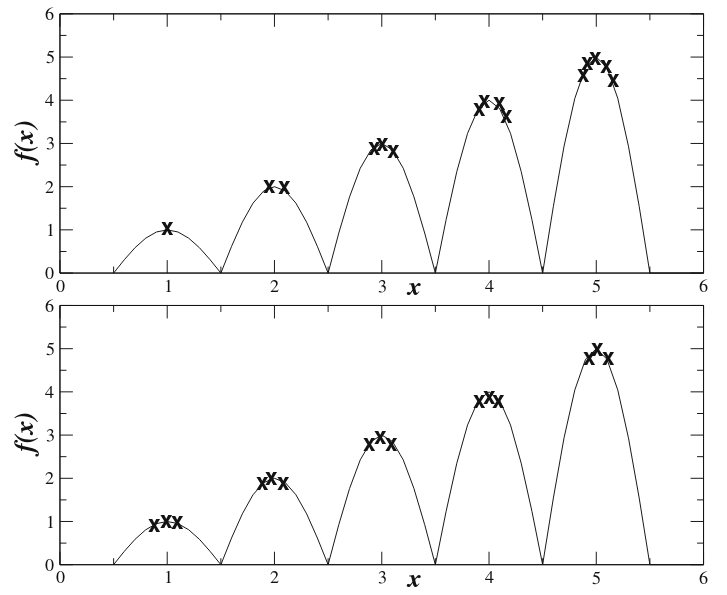
\includegraphics[width=0.45\textwidth]{images/fitness-sharing-vs-crowding}
    \caption{Idealised population distributions under fitness sharing (top)
    and crowding (bottom).
    There are five peaks in the landscape with fitnesses (5,4,3,2,1) and the population size is 15.
    Fitness sharing allocates individuals to peaks in proportion to their fitness, whereas crowding
    distributes the population evenly amongst the peaks.}\label{fitness-sharing-vs-crowding}
\end{figure}
Here, $d$ is the distance for which we re-used our Euclidean distance function. Details on the
sharing function $sh$ can be found in chapter 5.5.3 of the \book. There was a big drawback for our
EA using fitness sharing. As can be seen in \eqref{eq:fitness-sharing}, we need to calculate the
distance for each possible pairing in our population. For a population of size $n$, this requires
$n^2$ calculations. We can exploit the symmetry of the distance property, but that still leaves
$\tfrac{1}{2}n^2$ calculations, which can be a performance issue when $n$ becomes large. Because
the first results were hardly any better than a random search, we decided that this time
performance penalty (which seemed to matter for the online contest) was not worth the effort of
optimizing the fitness sharing method. Hence, we implemented a third method to overcome
multimodality.

\subsection{Island Model}
As a last approach, we implemented the \emph{island model} described in chapter 5.5.6 of the \book.
The main idea is very simple. Instead of keeping a single population, one keeps several
subpopulations in parallel. Ideally, every subpopulation explores a different region of the search
space. Every so many generations, a small number of individuals is exchanged amongst the islands,
to increase exploration when recombination happens between newcomers and inhabitants. When the
individuals
are migrated, they replace the worst individuals on the island of destination. Between
exchanges, the populations use the methods described in section \ref{sec:methodology} to exploit
their particular region of the search space. Table
\ref{tab:island-configuration} shows the configuration of our Island Model. Our EA improved
significantly on the Katsuura function. Instead of slightly outperforming a random search, this
method scored around $3$. We have experimented
with distinct settings for the different islands, but this did not improve the
performance further.
\begin{table}[t]
    \centering
    \begin{tabular}{|l|l|}
        \hline
        Islands & 5\\
        \hline
        Epoch length & 50 generations\\
        \hline
        Migration size & 5\\
        \hline
        Migration selection & Copy Best\\
        \hline
        Migration type & Effective Move\\
        \hline
    \end{tabular}
    \caption{Island Model configuration}\label{tab:island-configuration}
\end{table}


\section{Further Improvements}\label{sec:further-improvements}
Once the desired methods were implemented, the focus shifted to the parameters we used. The right
values for your parameters are very important for the performance of your EA. Some parameters, like
the epoch length and the migration size in the island model, were chosen based on the literature,
in this case the \book. Other parameter values were found by tuning.

\subsection{Parameter Tuning}
The most important parameters in our EA turned out to be the population size, and the mutation
parameters $\tau$, $\tau'$ and $\epsilon$. Since we had a limited number of evaluations, the bigger
the population the fewer generations we could create. We kept the population size therefore between
20-50 for each function, depending on the limit. The appropriate way to find the right values for
the remaining parameters would be through a grid search. However, due to time pressure we performed
most of
the tuning manually and recorded the results, keeping the best settings. We moved the mutation
parameters from their respective mutation functions to the global settings to be able the
distinguish between functions. The mutation parameters $\tau$ and $\tau'$ turned out to be tricky.
According to the literature we should set the $\tau$ values in our uncorrelated mutation with $n$
step sizes as follows: $\tau' \propto \frac{1}{\sqrt{2n}}$ and $\tau \propto
\frac{1}{\sqrt{2\sqrt{n}}}$.

Interestingly, when we experimented with proportionally different values, we acquired better
results. With the contest in mind, we decided to use the tuned parameter values: $\tau' \propto
\frac{1}{n}$ and $\tau \propto \frac{n}{10}$.

\subsection{Time dependent variables}
Another major change was the dependency on time for parameters. In the first generations one wants
to explore the search space, but after some time one might rather exploit the uncover high-fitness
regions. We used a self-adaptive mutation step size $\sigma$ which is bounded by some $\epsilon$
such that
\[
    \sigma < \epsilon \implies \sigma = \epsilon.
\]
We implemented a time dependency for the lower bound on the mutation step size. The result of this
is that in early stages mutation can be large so there is a lot of exploration, but in later stages
close to the evaluation limit the reduced lower bound allows for smaller mutations, such that the
high-fitness region can be exploited. This improvement bumped our performance on Katsuura to a
score of $8.5$. We planned to make the selection pressure time dependent as well, but we were not
able to implement this in time. We strongly believe this would have been a big improvement.


\section{Implementation}\label{sec:implementation}
In this section we will give a brief overview of the java specific choices that we made regarding
the implementation. All our code is available at our online repository \cite{github}.

\noindent We wanted to keep the main class as clean as possible. Therefore we created an
\mintinline{java}{Individual} class to store a candidate. We also created a seperate
\mintinline{java}{Population} class to store multiple \mintinline{java}{Individual}s. The
\mintinline{java}{Population} class also contains all the functions that implement the components
of the EA, except for mutation. The mutation operator works on individuals, so it made sense to put
all the mutation functions in the \mintinline{java}{Individual} class. Since we planned from the
beginning to implement a lot of different methods per EA component, we created an
\mintinline{java}{Options} class which can be passed to a \mintinline{java}{Population} object. The
\mintinline{java}{Options} class contains several \mintinline{java}{Enum} types to differentiate
between component methods, as well as some default parameter settings. This allowed us to easily
switch between methods. Lastly, we implemented a
separate \mintinline{java}{IslandModel} class, which in turn contains an array of
\mintinline{java}{Population} objects. To be as flexible as possible in our main class, both the
\mintinline{java}{Population} class and the \mintinline{java}{IslandModel} class implement a custom
\mintinline{java}{EAPopulation} interface, which specifies the basic EA components.

\section{Results \& Conclusion}
In figure \ref{fig:plot} you can see the results of our EA. The algorithm achieves a score of
$9.999977801879053 \pm 2.050283620022662\mathrm{e}{-05}$ on BentCigar, $8.893163092810429 \pm
0.38613823273700193$ on Katsuura and $9.783751107206767 \pm 0.5746303080312153$ on the Schaffers
function. These scores are the average over 25 runs, and the errors the corresponding standard
deviation. It shows our EA works well on the BentCigar and Schaffers functions, but less so on
Katsuura. From the boxplot its also clear that there is a much bigger variation in the scores
achieved on Katsuura. A possible cause is the multimodality of Katsuura: our probabilistic algorithm
has trouble finding the global maximum. This is also seen in the results for the Schaffers function:
the crystals shown in figure \ref{fig:plot} are the outliers.

\begin{figure}
\center{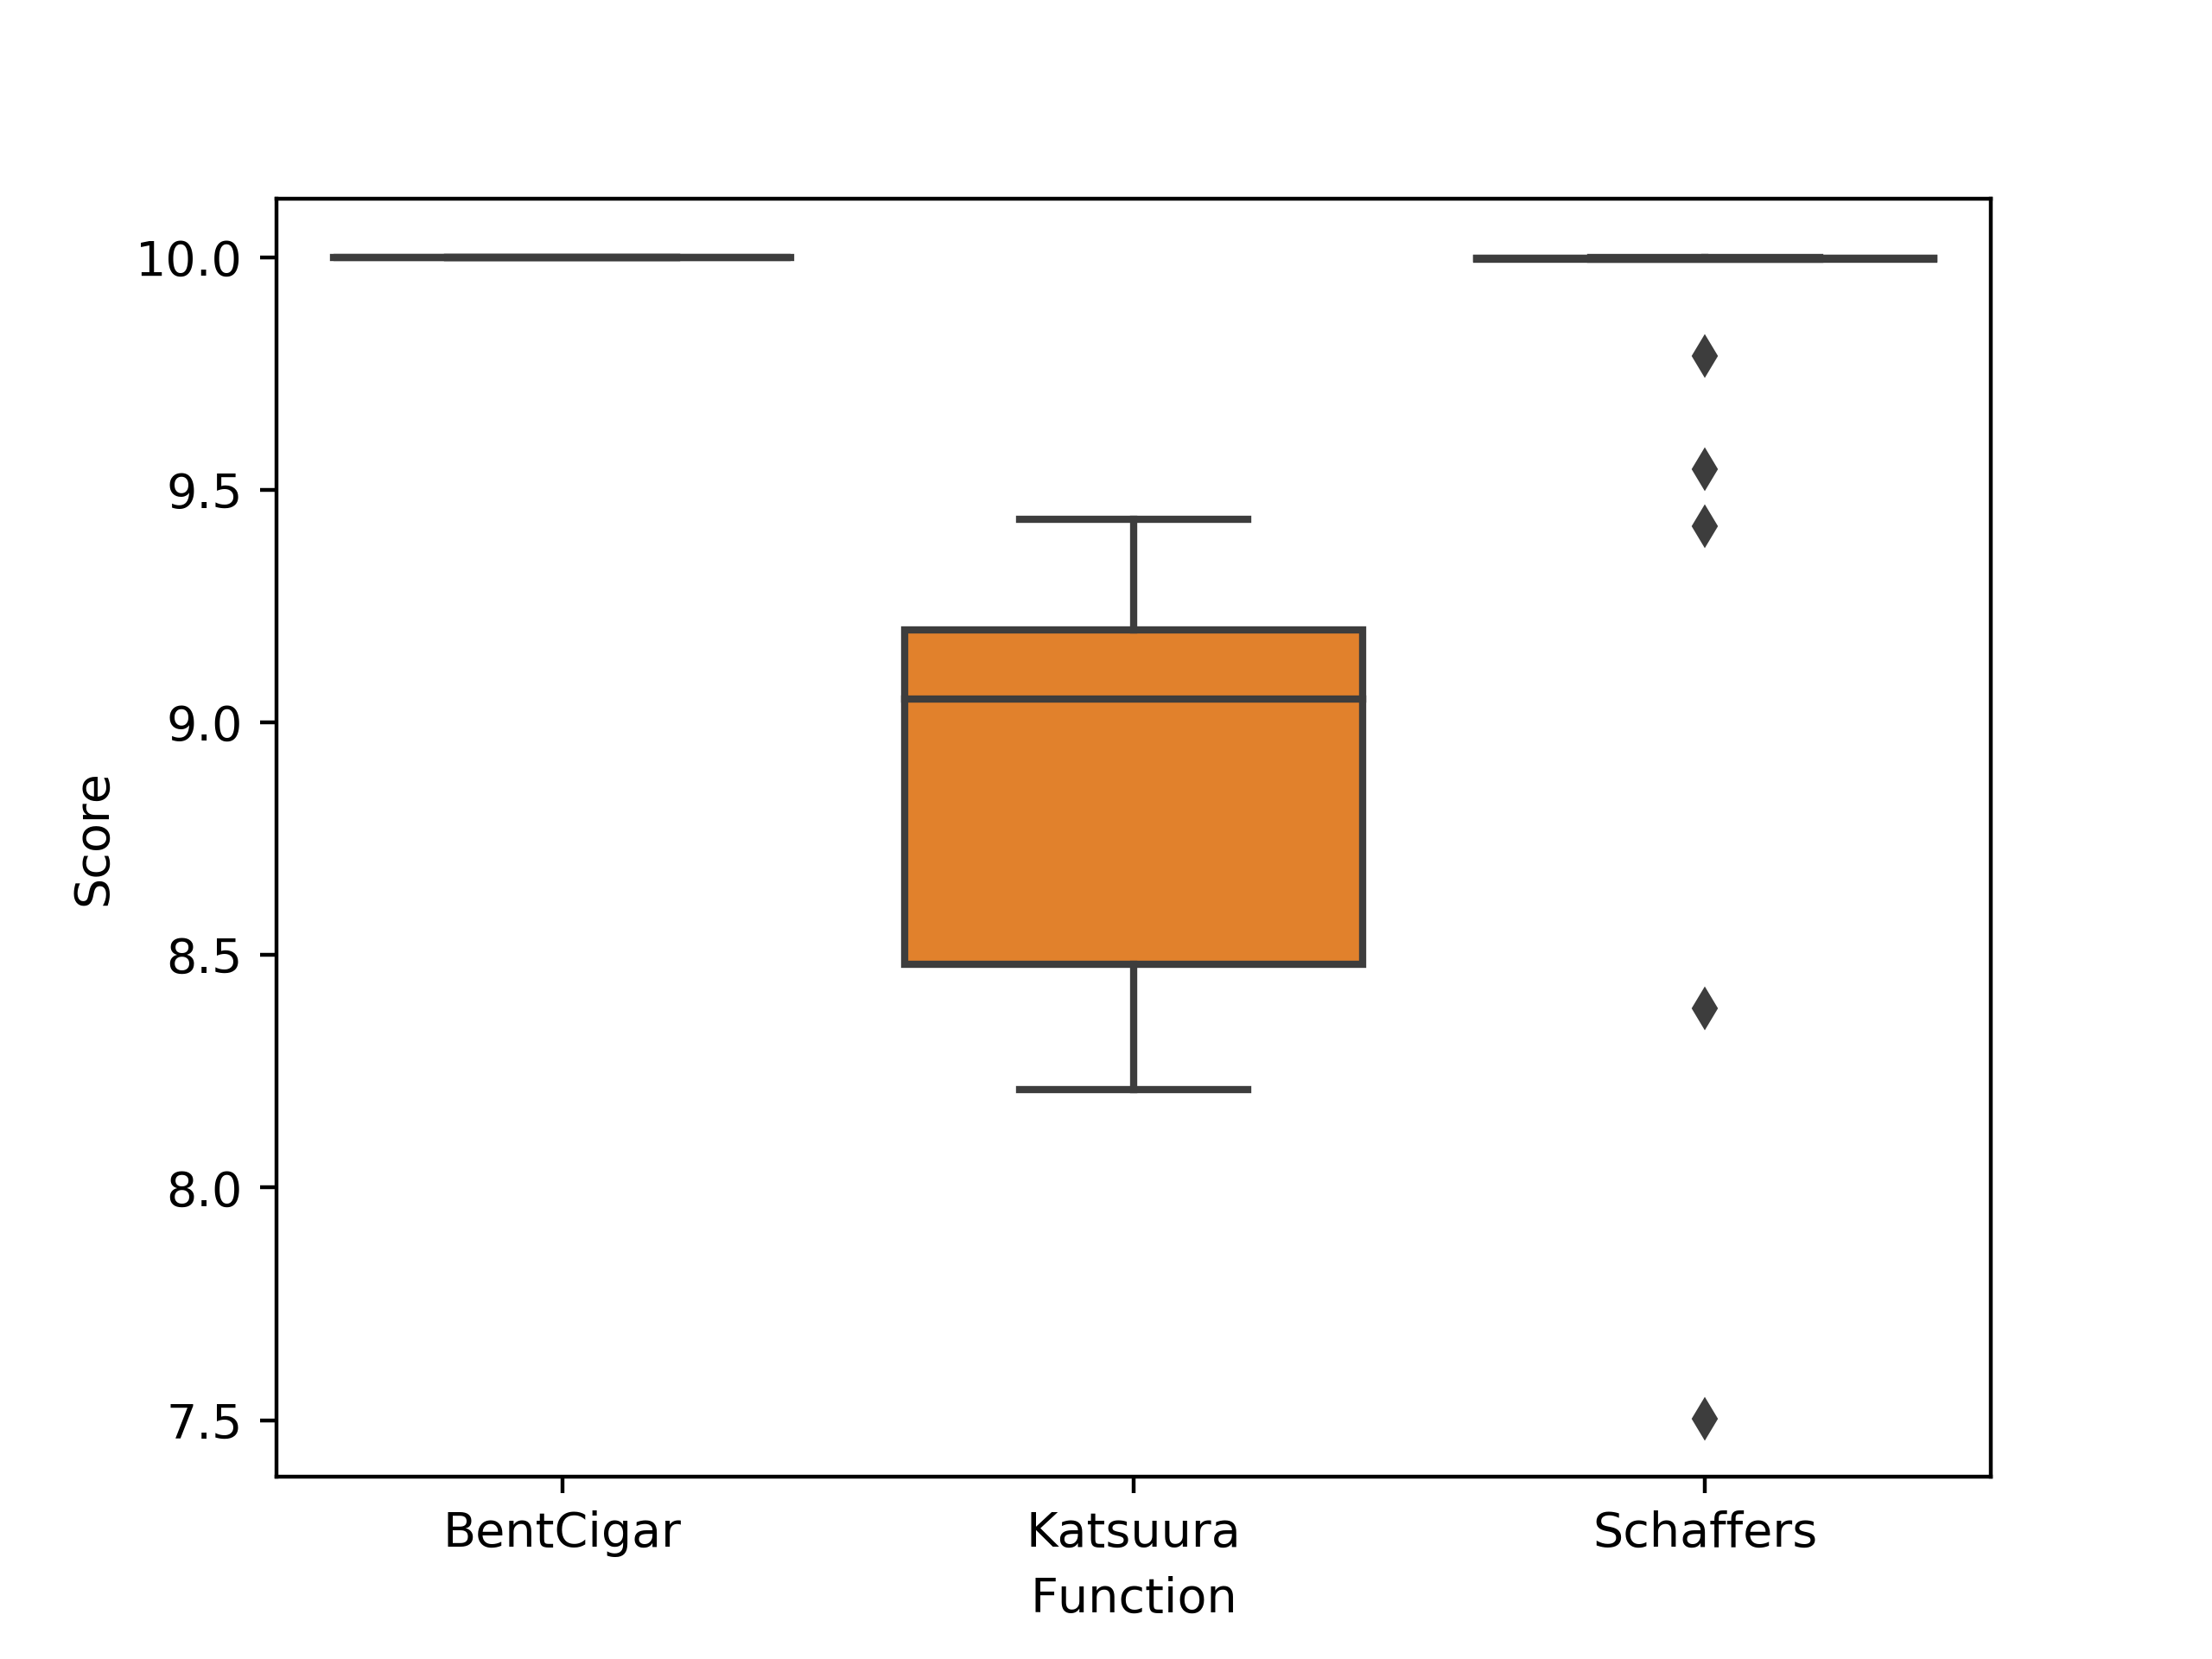
\includegraphics[height=7cm]{images/results_n25}}
\caption{A boxplot of the scores achieved by the EA on the three functions.}
\label{fig:plot}
\end{figure}

\section{Recommendations}
While experimenting with the recombination methods from section \ref{sec:recombination} we always
chose the recombination parameter $\alpha$ uniformly from $[0, 1]$. It would be interesting to also
experiment with constant values for $\alpha$, such as the commonly uses $\alpha = 0.5$.

As mentioned in section \ref{sec:mutation} we have an incomplete implementation of the ``Correlated
Mutations'' method where the only missing part is an import of a class from an external package. We
used a makefile to manage compiling the program. It could be worthwhile to learn how to use Maven, a
build tool specially crafted for use with Java programs \cite{wiki:maven}. We expect that this build
tool alleviates the problems one stumble upon when trying to use an external Java package.

Another recommendation is to have an extensive grid search for the optimal parameter values. Since
tuned mostly manually, we probably haven't found the best settings, which might be a reason why we
have not found the function maxima.

More sophisticated adaptation of variables as we did with the bound on the mutation step size woulc
probably have lead to better scores. An adaptive selection pressure would have been a very nice
improvement.

An idea left unexplored is prohibiting incest. The possible defects in offspring from incestuous
relations have been researched \cite{wiki:inbreeding}. It would be amusing to see if prohibiting
incest in our program would also lead to fitter individuals.

{\footnotesize\bibliographystyle{acm}
\bibliography{bibliography}}
\end{document}
